\documentclass{standalone}
\usepackage{tikz}
\usetikzlibrary[arrows,positioning,matrix]

\begin{document}
\begin{tikzpicture}
  \node[draw=none] (schematic) {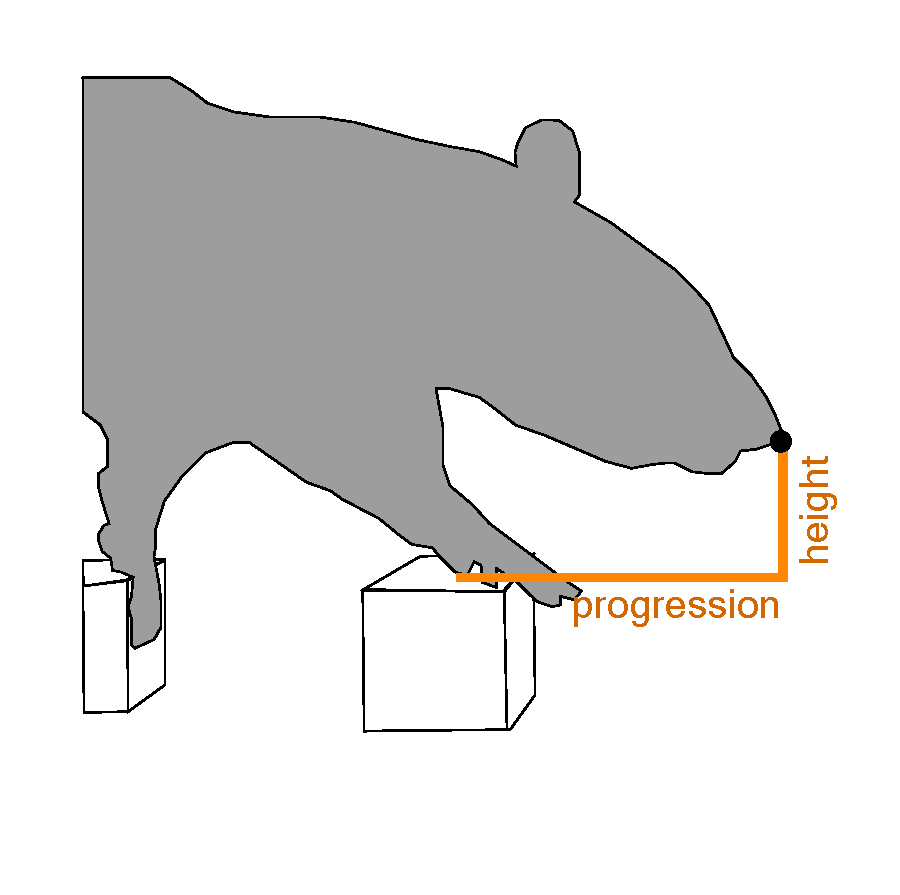
\includegraphics[width=0.5\textwidth]{elements/postureschematic}};
  \node[draw=none,above left=-5mm and -5mm of schematic] {A};

  \node[draw=none,right=1mm of schematic] (postureexample) {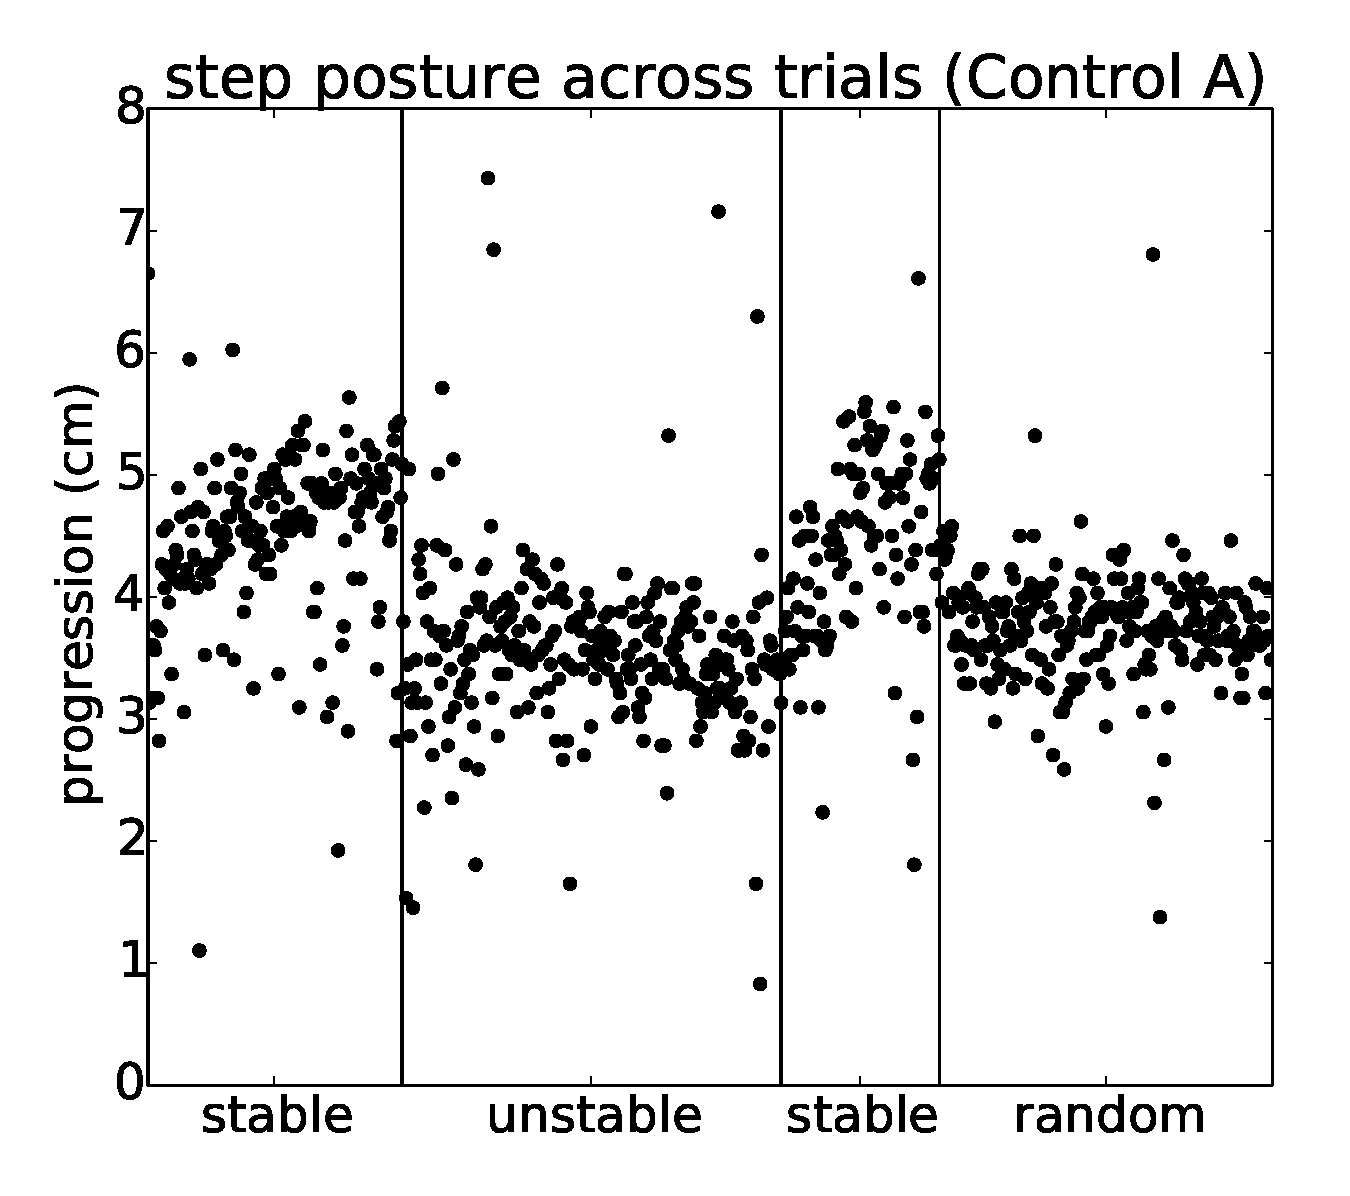
\includegraphics[width=0.5\textwidth]{elements/continuousposture}};
  \node[draw=none,above right=-5mm and 2mm of schematic] {B};
\end{tikzpicture}
\end{document}